%%%%%%%%%%%%%%%%%%%%%%%%%%%%%%%%%%%%%%%%%%%%%%%%%%%%%%%%%%%%%%%%%%%%%%%%%%%%%%%%%%%%%%%%%%%%%%%%%%%%%%%
%%%%%%%%%%%%%% Template de Artigo Adaptado para Trabalho de Diplomação do ICEI %%%%%%%%%%%%%%%%%%%%%%%%
%% codificação UTF-8 - Abntex - Latex -  							     %%
%% Autor:    Fábio Leandro Rodrigues Cordeiro  (fabioleandro@pucminas.br)                            %% 
%% Co-autor: Prof. João Paulo Domingos Silva  e Harison da Silva                                     %%
%% Revisores normas NBR (Padrão PUC Minas): Helenice Rego Cunha e Prof. Theldo Cruz                  %%
%% Versão: 1.0     13 de março 2014                                                                  %%
%%%%%%%%%%%%%%%%%%%%%%%%%%%%%%%%%%%%%%%%%%%%%%%%%%%%%%%%%%%%%%%%%%%%%%%%%%%%%%%%%%%%%%%%%%%%%%%%%%%%%%%

\section{\esp Implementação}

Para a implementação da solução foi utilizado uma adaptação do algoritmo de fluxo máximo Ford-Fulkerson \cite{site} onde foi definido o fluxo máximo como 1. Para cada rede de fluxo gerada faz-se uma busca em largura partindo do vértice s (vértice definido como origem do grafo) armazenamento em um vetor quais são os pais de cada vértice. Uma vez finalizada a busca precorre o vetor de pais partindo do vértice t (vértice definido como destino do grafo) adicionando o pai de cada vértice no começo de uma lista para definir qual foi o caminho percorrido pela busca. O método se repete até que a busca não consiga encontrar o vértice t e retorna um conjunto de de possíveis caminhos disjuntos de s para t.

O método foi implementado em Java utilizando o paradigma da orientação à objetos. Nesta implementação o grafo é um objeto que armazena em seu interior uma matriz de adjacência, o vértice de origem (s) e o vértice de destino (t), além do número total de vértices. A figura \ref{impl-grafo} mostra a implementação do código responsável por armazenar um grafo

\begin{figure}[H]
    \centering
    \caption{Implementação da classe grafo}
    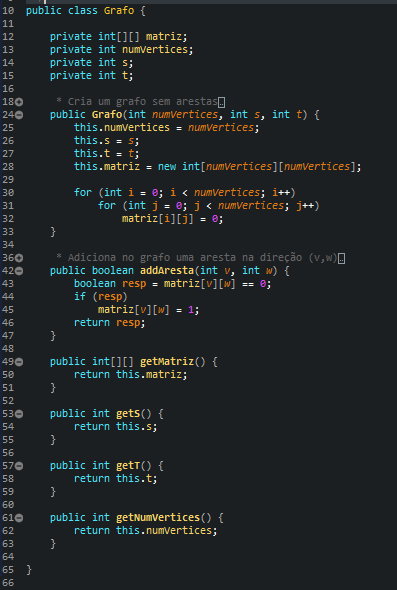
\includegraphics[width=0.6\textwidth]{figuras/grafoClass.png}
    \label{impl-grafo}
\end{figure}

A parte responsável por encontrar os caminhos conta com dois métodos, uma busca em largura que passa uma única vez em um vértice e que retorna um vetor indicando os pais de um vértice (Figura \ref{busca-largura}) e outro que a partir do vetor retornado pela busca monta os caminhos e gera uma nova rede de fluxo para realizar outra busca. O método só para quando a busca não encontra um caminho para t e retorna os caminhos encontrados (Figura \ref{encontrar-caminhos}).

\begin{figure}[H]
    \centering
    \caption{Implementação da busca em largura}
    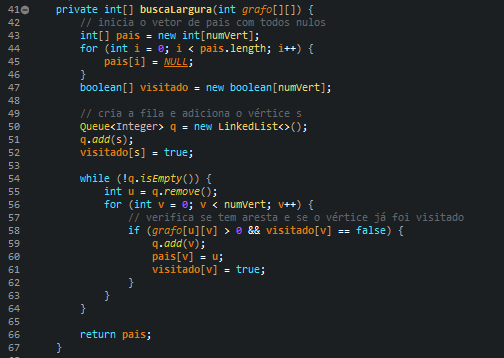
\includegraphics[width=0.7\textwidth]{figuras/buscaLargura.png}
    \label{busca-largura}
\end{figure}

\begin{figure}[H]
    \centering
    \caption{Implementação do método de encontrar caminhos}
    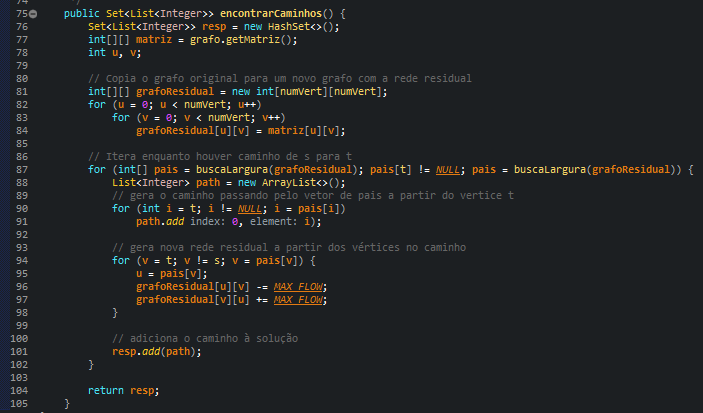
\includegraphics[width=0.7\textwidth]{figuras/encontrarCaminhos.png}
    \label{encontrar-caminhos}
\end{figure}

\section{\esp Testes e resultados}

Para os testes foram utilizados três grafos direcionados simples, isto é sem ciclos e sem arestas paralelas. Os grafos estavam salvos em aquivos de texto com  a seguinte estrutura:
na primeira linha o numero de vértices, o vértice de origem e o vértice de destino na respectiva ordem separados por espaços e nas linhas subsequentes  estava as arestas, uma em cada linha, com vértice de origem e vértice de destino nessa respectiva ordem separadas por espaços.

Os grafos testados foram os seguintes

\subsection{\esp Grafo 1}

O grafo G1 apresenta seis vértices e 11 arestas e os caminhos a serem procurados pelo algoritmo partiam do vértice 0 ao vértice 5 conforme a Figura \ref{grafo1}.
\begin{figure}[H]
	\centering	
	\caption[\hspace{0.1cm}]{G1}
	\vspace{-0.4cm}
	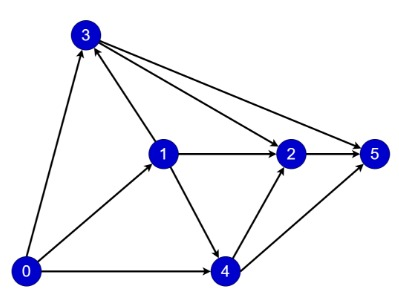
\includegraphics[width=0.6\textwidth]{figuras/grafo1.png}
	\label{grafo1}
\end{figure}
    
Para tal grafo existem no máximo três caminhos disjuntos conforme está marcado na Figura \ref{caminhos-grafo1} e, o método foi capaz de encontrar os três caminhos conforme indicado na Figura \ref{solucao-grafo1} extraída do console da IDE

\begin{figure}[H]
    \centering
    \caption{Caminhos disjuntos de G1}
    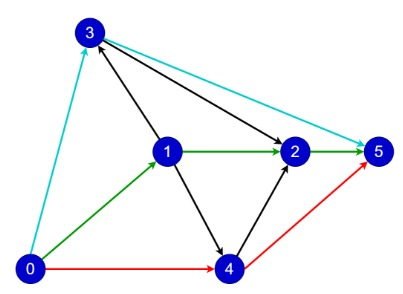
\includegraphics[width=0.6\textwidth]{figuras/caminhos-grafo1.png}
    \label{caminhos-grafo1}
\end{figure}


\begin{figure}[H]
    \centering
    \caption{Resultados de G1}
    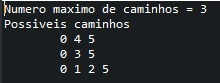
\includegraphics[width=0.6\textwidth]{figuras/solucao-grafo1.png}
    \label{solucao-grafo1}
\end{figure}
    
\subsection{\esp Grafo 2}

O grafo G2 apresenta nove vértices e 13 arestas e os caminhos a serem procurados pelo algoritmo partiam do vértice 0 ao vértice 8 conforme a Figura \ref{grafo2}

\begin{figure}[H]
    \centering
    \caption{G2}
    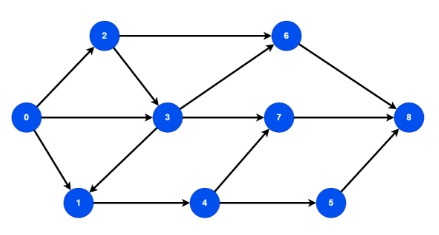
\includegraphics[width=0.6\textwidth]{figuras/grafo2.png}
    \label{grafo2}
\end{figure}

Para tal grafo existem no máximo três caminhos disjuntos conforme está marcado na Figura \ref{caminhos-grafo2} e, o método foi capaz de encontrar os três caminhos conforme indicado na Figura \ref{solucao-grafo2} extraída do console da IDE

\begin{figure}[H]
    \centering
    \caption{Caminhos disjuntos de G2}
    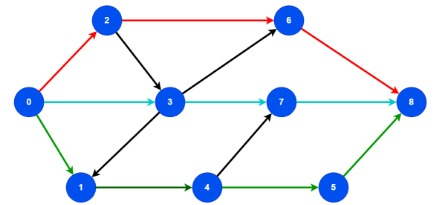
\includegraphics[width=0.6\textwidth]{figuras/caminhos-grafo2.png}
    \label{caminhos-grafo2}
\end{figure}


\begin{figure}[H]
    \centering
    \caption{Resultados de G2}
    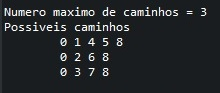
\includegraphics[width=0.6\textwidth]{figuras/solucao-grafo2.png}
    \label{solucao-grafo2}
\end{figure}
    
\subsection{\esp Grafo 3}

O grafo G3 apresenta 12 vértices e 21 arestas e os caminhos a serem procurados pelo algoritmo partiam do vértice 0 ao vértice 11 conforme a Figura \ref{grafo3}

\begin{figure}[H]
    \centering
    \caption{G3}
    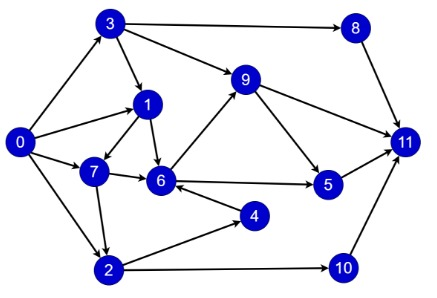
\includegraphics[width=0.6\textwidth]{figuras/grafo3.png}
    \label{grafo3}
\end{figure}

Para tal grafo existem no máximo três caminhos disjuntos conforme está marcado na Figura \ref{caminhos-grafo3} e, o método foi capaz de encontrar os três caminhos conforme indicado na Figura \ref{solucao-grafo3} extraída do console da IDE

\begin{figure}[H]
    \centering
    \caption{Caminhos disjuntos de G3}
    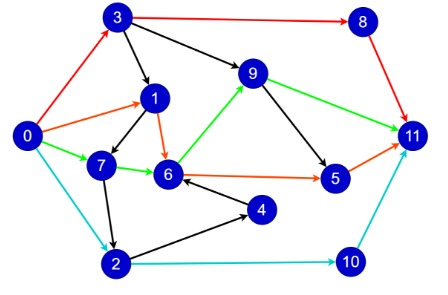
\includegraphics[width=0.6\textwidth]{figuras/caminhos-grafo3.png}
    \label{caminhos-grafo3}
\end{figure}


\begin{figure}[H]
    \centering
    \caption{Resultados de G3}
    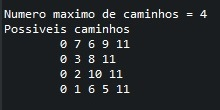
\includegraphics[width=0.6\textwidth]{figuras/solucao-grafo3.png}
    \label{solucao-grafo3}
\end{figure}



\section{\esp Conclusão}

Pode-se concluir que a solução implementada é capaz de achar possíveis caminhos disjuntos em grafos simples com um custo no pior caso de O(n), ou seja, o algoritmo é linear ao número de vértices de um grafo.